\subsection{Representación por bloques del vector de estado}

La primera decisión de diseño consiste en particionar el vector de estado en bloques contiguos e independientes. Cada bloque agrupa un subconjunto
de amplitudes adyacentes en memoria y se considera la unidad básica de compresión, descompresión, persistencia y reemplazo dentro del sistema. Con
esta organización, el vector deja de tratarse como un único arreglo monolítico y pasa a manejarse como una colección de fragmentos sobre los
cuales puede actuarse de manera localizada.

Esta decisión responde a una motivación tanto espacial como operacional. Desde el punto de vista de memoria, la compresión por bloques permite que
partes distintas del vector presenten ratios diferentes según su contenido efectivo. Desde el punto de vista del acceso, evita que una operación
que afecta solo una región reducida del estado obligue a descomprimir o recomprimir el arreglo completo. La granularidad del bloque se convierte
así en un parámetro central del diseño, ya que determina simultáneamente el potencial de compresión y el costo de recuperar datos para la
simulación.

La representación por bloques también favorece una integración más limpia con el simulador. En lugar de alterar la semántica de las operaciones
cuánticas, la arquitectura interpone una capa de almacenamiento que resuelve qué bloque contiene cada amplitud, cómo se recupera temporalmente y
cuándo debe volver a forma comprimida. Esto conserva el modelo de ejecución del simulador, pero reemplaza la idea de un vector siempre residente
en memoria densa por un backend capaz de administrar bloques en distintos estados de materialización.

\begin{figure}[H]
    \centering
    \caption{Particionamiento abstracto del vector de estado en bloques independientes}
    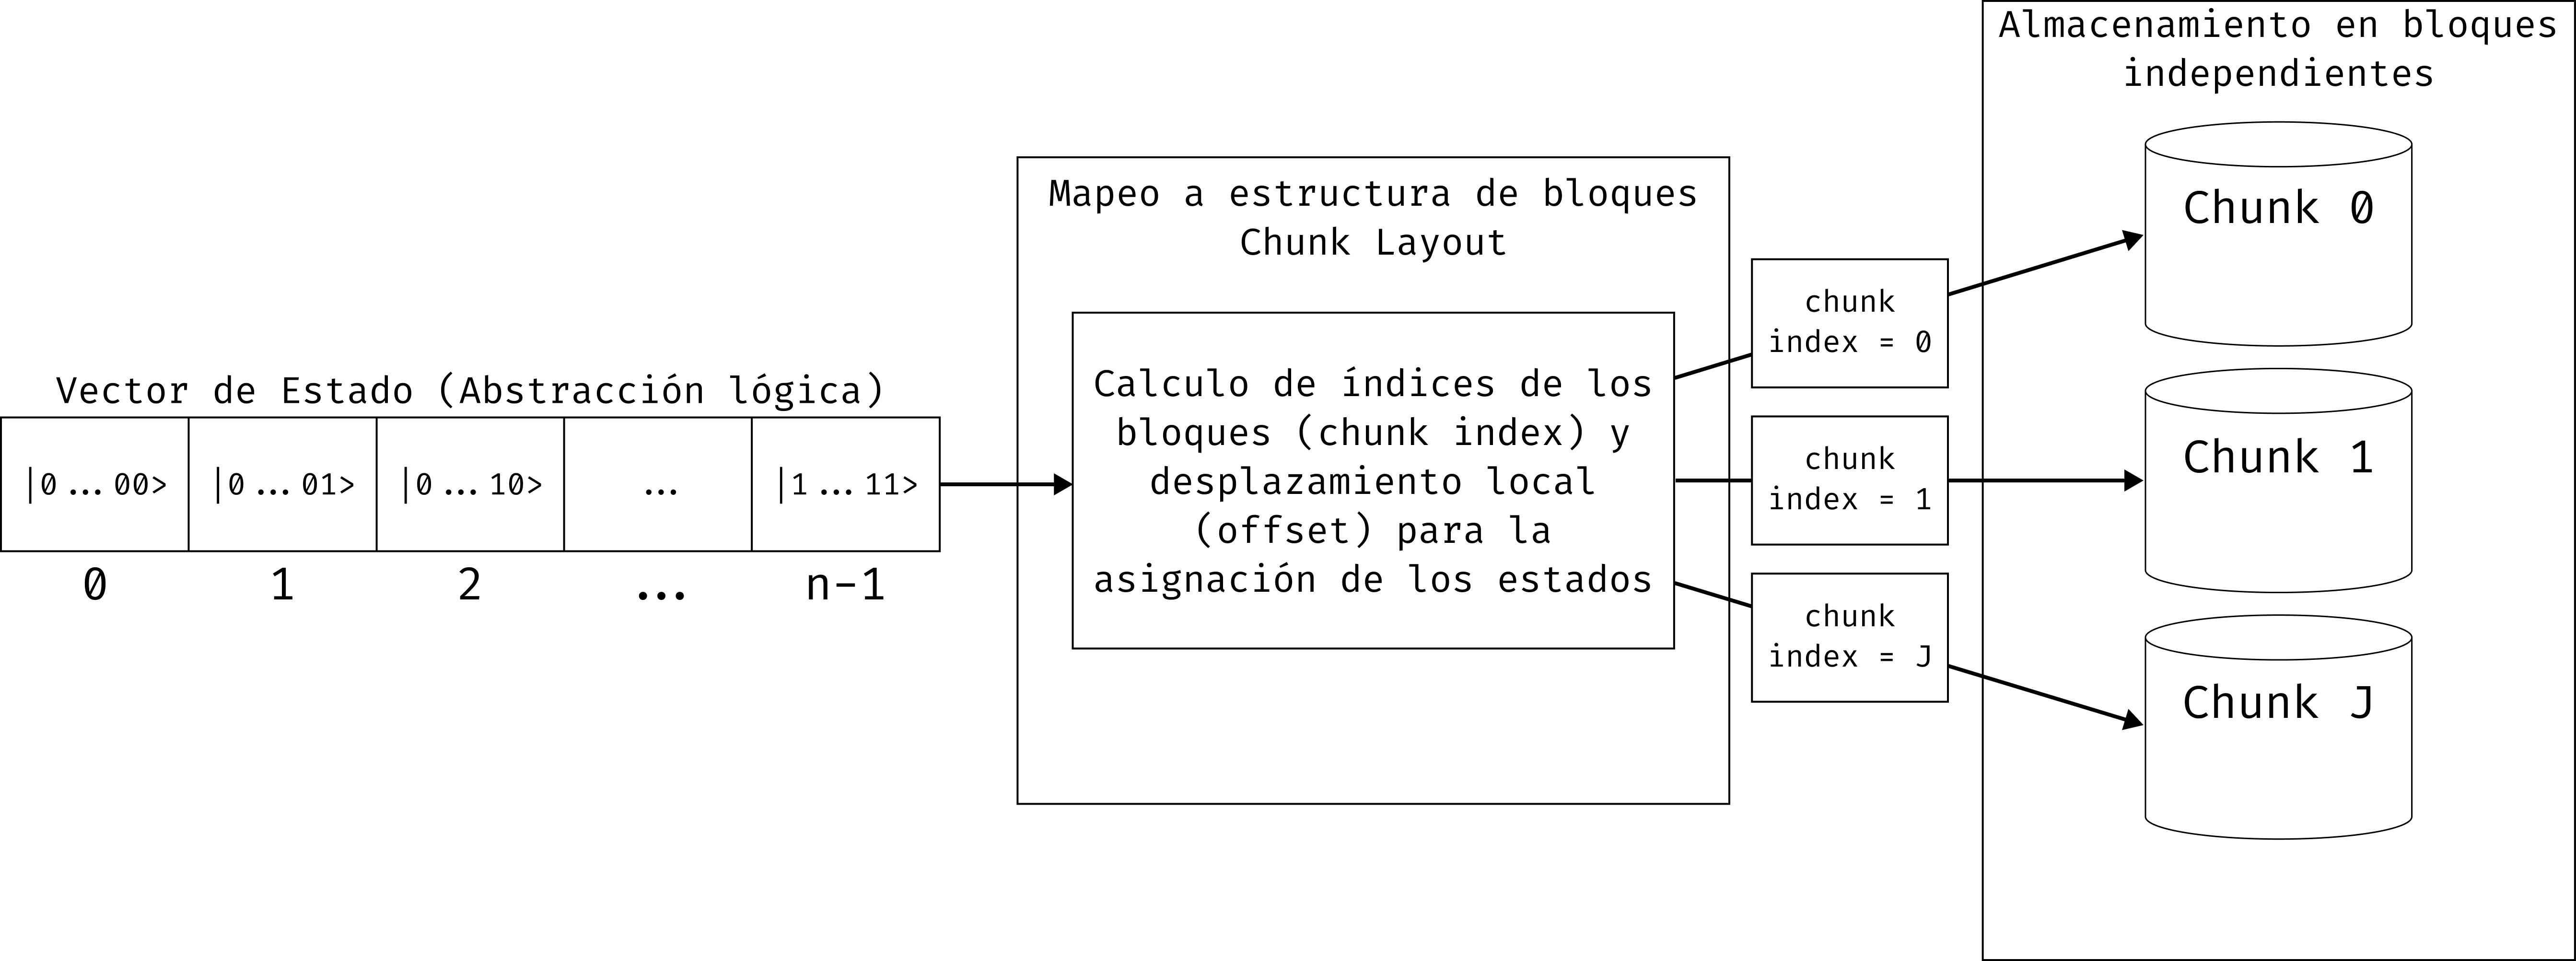
\includegraphics[width=1\textwidth]{images/simulation-design-blocks.png}
    \label{fig:simulation-design-blocks}
\end{figure}
